\subsection{实例:典型非周期信号的傅里叶变换}

\subsubsection{矩形脉冲信号}

\begin{theorem}
    设有一个脉高为 $E$,脉宽为 $\tau$ 的矩形脉冲信号 $f(t) = EG_{\tau}(t)$,
    则其傅里叶变换为
    \begin{align*}
        F(\omega) = \mathcal{F}[EG_{\tau}(t)] = E\tau\sa\left(\frac{\omega\tau}{2}\right),
    \end{align*}
    其幅度谱为 $|F(\omega)| = E\tau|\sa(\omega\tau/2)|$。
    $f(t)$ 和 $F(\omega)$ 的图像分别
    如图 \ref{fig:rectangular-pulse-signal} 和 \ref{fig:rectangular-pulse-signal-ft} 所示。
    \begin{figure}[H]
        \centering
        \begin{subfigure}{0.45\textwidth}
            \centering
            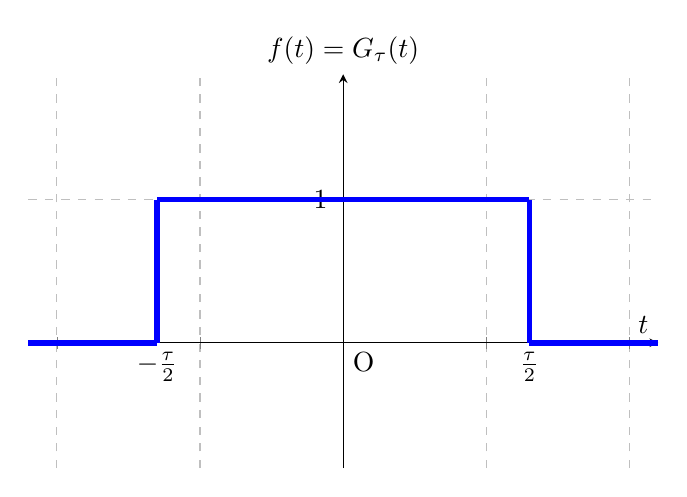
\begin{tikzpicture}
                \begin{axis}[
                    axis lines = middle,
                    xlabel = {$t$},
                    ylabel = {$f(t) = G_{\tau}(t)$},
                    ylabel style={at={(rel axis cs:0.5, 1)}, anchor=south},
                    xmin = -2.2, xmax = 2.2,
                    ymin = -0.2, ymax = 1.2,
                    xtick = {-2, -1, 0, 1, 2},
                    xticklabels = {$ $, $ $, $ $, $ $, $ $},
                    ytick distance = 1,
                    grid = major,
                    grid style = dashed,
                    scale only axis,
                    width = 8cm,
                    height = 5cm,
                    axis equal,
                ]
                \addplot[domain=-2.2:-1.3, samples=100, smooth, line width=2pt, blue] {0};
                \addplot[domain=-1.3:1.3, samples=100, smooth, line width=2pt, blue] {1};
                \addplot[domain=1.3:2.2, samples=100, smooth, line width=2pt, blue] {0};
                \addplot[smooth, line width=2pt, blue] coordinates {(-1.3, 0) (-1.3, 1)};
                \addplot[smooth, line width=2pt, blue] coordinates {(1.3, 1) (1.3, 0)};
                \node at (axis cs:0, 0) [anchor=north west] {O};
                \node at (axis cs:-1.3, 0) [anchor = north] {$-\frac{\tau}{2}$};
                \node at (axis cs:1.3, 0) [anchor = north] {$\frac{\tau}{2}$};
                \end{axis}
            \end{tikzpicture}
            \caption{$f(t)$ 的波形描述}
            \label{fig:rectangular-pulse-signal}
        \end{subfigure}
        \hfill
        \begin{subfigure}{0.45\textwidth}
            \centering
            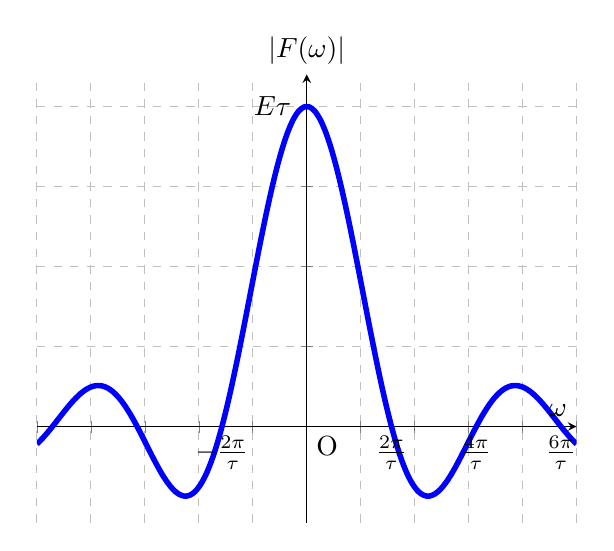
\begin{tikzpicture}
                \begin{axis}[
                    axis lines = middle,
                    xlabel = {$\omega$},
                    ylabel = {$|F(\omega)|$},
                    ylabel style={at={(rel axis cs:0.5, 1)}, anchor=south},
                    xmin = -10, xmax = 10,
                    ymin = -0.3, ymax = 1.1,
                    xtick = {-10, -8, -6, -4, -2, 0, 2, 4, 6, 8, 10},
                    xticklabels = {$ $, $ $, $ $, $ $, $ $, $ $, $ $, $ $, $ $, $ $, $ $},
                    ytick = {0, 0.25, 0.5, 0.75, 1},
                    yticklabels = {$ $, $ $, $ $, $ $, $E\tau$},
                    grid = major,
                    grid style = dashed,
                ]
                \addplot[domain=-10:10, samples=100, smooth, line width=2pt, blue] {sin(deg(x))/x};
                \node at (axis cs:0, 0) [anchor=north west] {O};
                \node at (axis cs:3.14, 0) [anchor = north] {$\frac{2\pi}{\tau}$};
                \node at (axis cs:-3.14, 0) [anchor = north] {$-\frac{2\pi}{\tau}$};
                \node at (axis cs:6.28, 0) [anchor = north] {$\frac{4\pi}{\tau}$};
                \node at (axis cs:9.42, 0) [anchor = north] {$\frac{6\pi}{\tau}$};
                \end{axis}
            \end{tikzpicture}
            \caption{$F(\omega)$ 的波形描述}
            \label{fig:rectangular-pulse-signal-ft}
        \end{subfigure}
        \caption{矩形脉冲信号及其傅里叶变换}
      \end{figure}
\end{theorem}

\begin{proof}
    由傅里叶变换的定义,有
    \begin{align*}
        F(\omega) & = \int_{-\infty}^{+\infty}EG_{\tau}(t)\mathe^{-\mathi\omega t}\D{t} \\
        & = E\int_{-\tau/2}^{\tau/2}\mathe^{-\mathi\omega t}\D{t} \\
        & = E\left.\frac{\mathe^{-\mathi\omega t}}{-\mathi\omega}\right|_{-\tau/2}^{\tau/2} \\
        & = \frac{E}{-\mathi\omega}\left(\mathe^{-\mathi\omega\tau/2} - \mathe^{\mathi\omega\tau/2}\right) \\
        & = \frac{E\cdot (-2\mathi\sin(\omega\tau/2))}{-\mathi\omega} \\
        & = E\tau\sa\left(\frac{\omega\tau}{2}\right).
    \end{align*}
    命题得证。
\end{proof}

\begin{property}[矩形脉冲信号的 FT 的特点]
    矩形脉冲信号的 FT 具有以下特点:
    \begin{itemize}
        \item FT 为 $\sa$ 函数,原点处函数值为矩形脉冲的面积 $E\tau$。
        \item FT 的零点为 $\omega = 2k\pi / \tau(k \in \set{Z}, k \neq 0)$。
        \item 频域的能量集中在第一个过零点区间,$[-2\pi/\tau, 2\pi/\tau]$。
        \item 带宽为 $B_\omega = 4\pi / \tau$,只与脉宽有关,与脉高无关。
    \end{itemize}
\end{property}

\subsubsection{冲激信号}

\begin{theorem}
    设有一个冲激信号 $f(t) = E\delta(t)$,则其傅里叶变换为
    \begin{align*}
        F(\omega) = \mathcal{F}[E\delta(t)] = E.
    \end{align*}
\end{theorem}

\begin{proof}
    由傅里叶变换的定义,有
    \begin{align*}
        F(\omega) & = \int_{-\infty}^{+\infty}E\delta(t)\mathe^{-\mathi\omega t}\D{t} \\
        & = E\mathe^{-\mathi\omega\cdot 0} \\
        & = E.
    \end{align*}
    命题得证。
\end{proof}

\begin{remark}
    上述结论也可以由矩形脉冲信号的极限情况得到。

    当脉宽 $\tau$ 逐渐变窄时,其频谱必然展宽。
    可以想象:$\delta(t)$ 积分为 $1$,因此需要 $E\tau = 1$。
    若 $\tau \to 0$,这时矩形脉冲就变成了 $\delta(t)$,
    其相应频谱 $F(\omega)$ 必定等于常数 $1$。
\end{remark}

\begin{definition}[均匀谱]
    冲激函数的频谱等于常数,即在整个频率范围内频谱是均匀分布的。
    
    显然,在时域中变化异常剧烈的冲激函数中包含了\bd{幅度相等}的\bd{所有}频率分布。
    因此,这种频谱常被称为\bd{均匀谱},或\bd{白色谱}。
\end{definition}

\begin{theorem}[常数的傅里叶变换]
    常数信号 $f(t) = E$ 的傅里叶变换为
    \begin{align*}
        F(\omega) = \mathcal{F}[E] = 2\pi\cdot E\delta(\omega).
    \end{align*}
    特别地,$\mathcal{F}[1/2\pi] = \delta(\omega), \mathcal{F}[1] = 2\pi\delta(\omega)$。
    这说明,直流信号的傅里叶频谱是位于零点的冲激函数。

    反之,冲激信号 $F(\omega) = E\delta(\omega)$ 的傅里叶逆变换为
    \begin{align*}
        f(t) = \mathcal{F}^{-1}[E\delta(\omega)] = \frac{E}{2\pi}.
    \end{align*}
    这说明,频谱零点处的冲激函数来自信号的直流分量。
\end{theorem}

\begin{proof}
    由于 $F[\mathe^{\mathi \omega_0 t}] = 2\pi\delta(\omega - \omega_0)$,
    故当 $\omega_0 = 0$ 时,有
    \begin{align*}
        F[1] = 2\pi\delta(\omega).
    \end{align*}
    又因为傅里叶变换是线性的,故有
    \begin{align*}
        F[E] = E\cdot F[1] = 2\pi\cdot E\delta(\omega).
    \end{align*}
    反之,由傅里叶逆变换的定义,有
    \begin{align*}
        f(t) = \mathcal{F}^{-1}[E\delta(\omega)] = \frac{E}{2\pi}.
    \end{align*}
    命题得证。
\end{proof}

\subsubsection{符号函数}

\begin{note}
    此节属于自己额外整理的内容,不在课程范围内。
\end{note}

\begin{theorem}
    设有一个符号函数 $f(t) = \sgn{t}$,则其傅里叶变换为
    \begin{align*}
        F(\omega) = \mathcal{F}[\sgn{t}] = \frac{2}{\mathi\omega}.
    \end{align*}
\end{theorem}

\begin{note}
    如果我们用傅里叶变换的定义来计算 $\sgn{t}$ 的傅里叶变换,我们会发现
    \begin{align*}
        F(\omega) & = \int_{-\infty}^{+\infty}\sgn{t}\mathe^{-\mathi\omega t}\D{t} \\
        & = - \int_{-\infty}^{0}\mathe^{-\mathi\omega t}\D{t} + \int_{0}^{+\infty}\mathe^{-\mathi\omega t}\D{t} \\
    \end{align*}
    这两个积分是不收敛的,因此我们需要用其他方法来计算 $\sgn{t}$ 的傅里叶变换。
\end{note}

\begin{proof}
    考虑使用指数函数信号来逼近符号函数,即
    \begin{align*}
        f_a(t) = \begin{cases}
            \mathe^{-at}, & t \ge 0, \\
            -\mathe^{at}, & t < 0,
        \end{cases}
        \quad a > 0.
    \end{align*}
    则符号函数可以表示为
    \begin{align*}
        \sgn{t} = \lim_{a \to 0^+}f_a(t).
    \end{align*}
    我们首先计算 $f_a(t)$ 的傅里叶变换:
    \begin{align*}
        F_a(\omega) & = \int_{-\infty}^{+\infty}f_a(t)\mathe^{-\mathi\omega t}\D{t} \\
        & = \int_{0}^{+\infty}\mathe^{-at}\mathe^{-\mathi\omega t}\D{t} + \int_{-\infty}^{0}-\mathe^{at}\mathe^{-\mathi\omega t}\D{t} \\
        & = \int_{0}^{+\infty}\mathe^{-(a + \mathi\omega)t}\D{t} - \int_{-\infty}^{0}\mathe^{(a - \mathi\omega)t}\D{t} \\
        & = \left.\frac{\mathe^{-(a + \mathi\omega)t}}{-(a + \mathi\omega)}\right|_{0}^{+\infty} - \left.\frac{\mathe^{(a - \mathi\omega)t}}{a - \mathi\omega}\right|_{-\infty}^{0} \\
        & = \frac{1}{a + \mathi\omega} - \frac{1}{a - \mathi\omega} \\
        & = -\frac{2\mathi\omega}{a^2 + \omega^2}.
    \end{align*}
    因此,有
    \begin{align*}
        F(\omega) = \lim_{a \to 0^+}F_a(\omega) = \lim_{a \to 0^+}\left(-\frac{2\mathi\omega}{a^2 + \omega^2}\right) = \frac{2}{\mathi\omega}.
    \end{align*}
    命题得证。
\end{proof}

\subsubsection{单位阶跃函数}

\begin{theorem}
    \label{thm:unit-step-function-ft}
    设有一个单位阶跃函数 $f(t) = u(t)$,则其傅里叶变换为
    \begin{align*}
        F(\omega) = \mathcal{F}[u(t)] = \frac{1}{\mathi\omega} + \pi\delta(\omega).
    \end{align*}
\end{theorem}

\begin{proof}
    由于
    \begin{align*}
        u(t) = \frac{1 + \sgn{t}}{2},
    \end{align*}
    故由傅里叶变换的线性性质,有
    \begin{align*}
        F(\omega) = \frac{1}{2}\mathcal{F}[1] + \frac{1}{2}\mathcal{F}[\sgn{t}] = \frac{1}{2}\cdot 2\pi\delta(\omega) + \frac{1}{2}\cdot \frac{2}{\mathi\omega} = \frac{1}{\mathi\omega} + \pi\delta(\omega).
    \end{align*}
    命题得证。
\end{proof}
